% ===========================================================================
% fig-cost-solve.tex — cost-per-solve vs solve-rate scatter, with the
% kimi<->opus blind-mixing line.
% BODY ONLY (tikzpicture). Wrapper/caption/label live in the section file.
% Requires % ===========================================================================
% fig-style.tex — shared colour / marker scheme for EVERY main-paper figure.
% \input this ONCE from the preamble of main.tex (after tikz + pgfplots).
%
% House rule: the palette is defined here and nowhere else. Each series also
% gets a distinct marker AND line style so the figures survive grayscale
% printing.
%
%   \sysname / deployed .. cSys   (blue!70!black)    mark *
%   opus / claude ........ cOpus  (red!70!black)     mark square*
%   gpt .................. cGpt   (teal!70!black)    mark triangle*
%   kimi ................. cKimi  (violet!70!black)  mark diamond*
%   flash ................ cFlash (orange!70!black)  mark pentagon*
%   greedy / baseline .... cBase  (gray)             mark o
% ===========================================================================
% The pipeline diagram needs the calc library for coordinate arithmetic; the
% rest of the libraries are already loaded in main.tex's preamble.
\usetikzlibrary{calc}
% Hatching, so bar charts stay readable in grayscale.
\usetikzlibrary{patterns}

\colorlet{cSys}{blue!70!black}
\colorlet{cOpus}{red!70!black}
\colorlet{cGpt}{teal!70!black}
\colorlet{cKimi}{violet!70!black}
\colorlet{cFlash}{orange!70!black}
\colorlet{cBase}{gray}

% Common axis furniture: footnotesize ticks/legend, small titles, framed
% legend in gray!50, light horizontal grid.
\pgfplotsset{
  paperaxis/.style={
    width=0.80\linewidth,
    height=5.2cm,
    tick label style={font=\footnotesize},
    label style={font=\footnotesize},
    title style={font=\small},
    legend style={font=\footnotesize, draw=gray!50, fill=white,
                  fill opacity=0.9, text opacity=1, rounded corners=1pt},
    every axis plot/.append style={line width=0.7pt},
    grid style={gray!25, line width=0.3pt},
    axis line style={gray!60},
    tick style={gray!60},
  },
  papermark/.style={mark size=2.6pt},
}
 in the preamble.
% Provenance: data/receipts/outcomes_per_task.json and
%             data/receipts/routing_scenarios.json.
%
% Design notes:
%   - The router point and the no-router ablation differ by $0.003 per solve,
%     under 1.5pt on this log axis, so they share ONE composite glyph (open
%     cKimi diamond for the ablation, smaller filled cSys disc drawn last
%     inside it) with one colour-keyed callout and one leader; two markers
%     would misstate the resolution of the figure.
%   - The mixing reference is convex in LINEAR cost, so it is sampled as the
%     true mixture and renders as a curve on a log-x axis.
% ===========================================================================
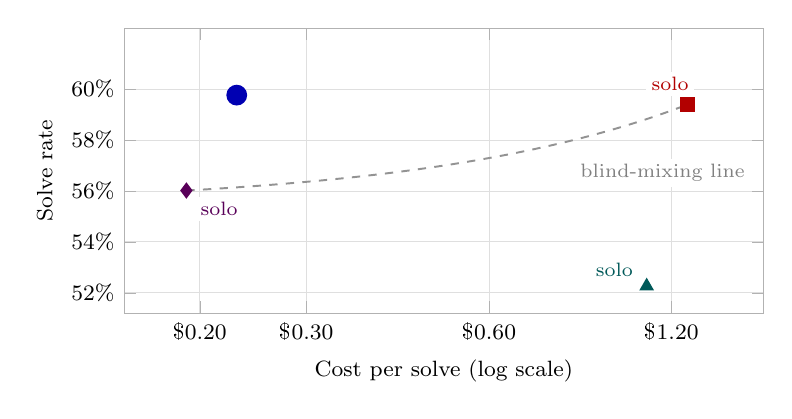
\begin{tikzpicture}
\begin{axis}[
  paperaxis,
  xmode=log,
  log basis x=10,
  xmin=0.150, xmax=1.70,
  ymin=51.2, ymax=62.4,
  xtick={0.2,0.3,0.6,1.2},
  xticklabels={\$0.20,\$0.30,\$0.60,\$1.20},
  log ticks with fixed point,
  xminorticks=false,
  ytick={52,54,56,58,60},
  yticklabel={\pgfmathprintnumber{\tick}\%},
  xlabel={Cost per solve (log scale)},
  ylabel={Solve rate},
  ymajorgrids=true,
  xmajorgrids=true,
]

% --- blind-mixing locus: kimi -> opus (reference, deliberately subdued) --
% Solve rate is affine in LINEAR cost, so on a log-x axis this is a CURVE,
% not a straight segment; drawing it straight would overstate the baseline.
% Sampled densely; the endpoints are exactly the two solo points.
\addplot[dashed, line width=0.7pt, color=cBase!85, mark=none, forget plot,
         domain=0.190:1.274, samples=120, smooth]
  {56.02 + (x-0.190)*(59.40-56.02)/(1.274-0.190)};

% --- solo anchors (context) ---------------------------------------------
\addplot[only marks, mark size=2.4pt, color=cOpus, mark=square*, forget plot]
  coordinates {(1.274,59.40)};
\addplot[only marks, mark size=2.4pt, color=cKimi, mark=diamond*, forget plot]
  coordinates {(0.190,56.02)};
\addplot[only marks, mark size=2.4pt, color=cGpt, mark=triangle*, forget plot]
  coordinates {(1.091,52.26)};

% --- \sysname (protagonist): larger mark, drawn last, on top ------------
% The no-router ablation is deliberately NOT plotted here; it lives in the
% main results table. The figure carries the headline only.
\addplot[only marks, mark size=3.3pt, color=cSys, mark=*,
         mark options={fill=cSys, draw=cSys, line width=0.9pt}, forget plot]
  coordinates {(0.230,59.77)};
\node[font=\scriptsize, color=cSys, anchor=south, inner sep=1.5pt, fill=white]
  at (axis cs:0.230,60.05) {\textbf{\sysname}};

% --- inline labels ------------------------------------------------------
% Placement rule: each label is anchored so its box lies in a quadrant no
% marker, no grid tick and no segment of the dashed line passes through.
\node[font=\scriptsize, color=cOpus, anchor=south east, inner sep=2pt, fill=white]
  at (axis cs:1.310,59.70) {\fxopusS solo};
\node[font=\scriptsize, color=cKimi, anchor=north west, inner sep=2pt, fill=white]
  at (axis cs:0.196,55.80) {\fxkimiS solo};
\node[font=\scriptsize, color=cGpt, anchor=south east, inner sep=2pt, fill=white]
  at (axis cs:1.060,52.40) {\fxgptS solo};
\node[font=\scriptsize, color=cBase, anchor=north east, inner sep=2pt, fill=white]
  at (axis cs:1.620,57.30) {blind-mixing line};

\end{axis}
\end{tikzpicture}
